\chapter{Resultados}\label{cap:resultados}

Este capítulo apresenta os resultados dos módulos alterados. O termo de comparação é a \emph{baseline} do desafio SoccerNet-GSR \citep{somers2024soccernet}, executada com os seus módulos originais nos mesmos vídeos e no mesmo ambiente que o sistema proposto. Os dois sistemas partilham a deteção, o \emph{tracking}, a calibração e o modelo de reidentificação. Avaliam, por isso, os mesmos \emph{tracklets}, e as diferenças nos resultados são atribuídas ao que foi alterado. Para que a calibração fosse de facto igual nos dois, a calibração da \emph{baseline} foi refeita com uma homografia por \emph{frame}, pelas razões descritas na Secção~\ref{sec:res_calib_defeito}. A avaliação usa os três subconjuntos anotados, com $49$ vídeos de teste, $53$ de validação e $57$ de treino, $159$ no total. O SNGS-096, da validação, ficou de fora, porque a calibração falha nele nos dois sistemas.

O capítulo começa por avaliar cada módulo individualmente, com uma métrica própria e a inspeção visual descrita na Secção~\ref{sec:protocolo}. Depois, o GS-HOTA mede o efeito das alterações no sistema como um todo. A última secção compara o tempo de execução de cada módulo nos dois sistemas. Nenhuma regra nem limiar foi escolhido com o conjunto de treino, que serviu só para confirmar cada alteração (Secção~\ref{sec:ambiente}).

\section{Reconhecimento do Número da Camisola}\label{sec:res_jnr}

Para avaliar este módulo, conta-se a percentagem de \emph{tracklets} que recebem o número certo, ou seja, a exatidão por \emph{tracklet}. Para isso é preciso saber, primeiro, a que jogador da anotação de referência corresponde cada \emph{tracklet}. Em cada \emph{frame}, cada deteção do \emph{tracklet} fica associada à caixa anotada com que mais se sobrepõe, desde que o IoU seja de pelo menos $0.30$. O IoU (\emph{intersection over union}) é a área da interseção das duas caixas a dividir pela área da sua união. Cada \emph{tracklet} corresponde ao jogador associado em mais \emph{frames}. Por exemplo, se $90$ das $100$ deteções de um \emph{tracklet} coincidirem com o jogador anotado com o $7$, o \emph{tracklet} só está certo se o sistema lhe atribuir o $7$. Um \emph{tracklet} sem número atribuído conta como errado.

Só entram na avaliação os \emph{tracklets} com pelo menos cinco \emph{frames} que correspondem a um jogador com número anotado. Esse jogador tem de estar associado a pelo menos $30\%$ dos \emph{frames} do \emph{tracklet}, para excluir \emph{tracklets} que só de passagem se sobrepõem a ele. Ficam ainda de fora os \emph{tracklets} em que o \emph{tracker} trocou de identidade a meio, isto é, aqueles em que menos de $80\%$ das associações vão para o mesmo jogador. Num \emph{tracklet} que começa no $7$ e acaba no $10$ não há um único número certo. A \emph{baseline} e o sistema proposto são avaliados com estes critérios e sobre os mesmos \emph{tracklets}, pelo que o total avaliado é igual nos dois e a comparação é direta.

\subsection{Resultados}\label{sec:res_jnr_resultados}

Os valores desta secção são os da versão final do módulo. Nesta versão, o Qwen2.5-VL lê o número de cada \emph{tracklet} em janelas de recortes consecutivos, e cada leitura traz a confiança com que o modelo a fez. Só as leituras com confiança de pelo menos $0.5$ contam como voto, e o \emph{tracklet} recebe o número mais votado (Secção~\ref{sec:met-jnr-confianca}). A Secção~\ref{sec:res_jnr_confianca} compara esta versão com a primeira, que não usava a confiança e decidia apenas pela contagem de votos. A Tabela~\ref{tab:jnr} resume os resultados. A exatidão mais do que duplica nos três subconjuntos. Sobe de $19.2\%$ para $46.8\%$ no teste, de $15.8\%$ para $41.8\%$ na validação e de $12.0\%$ para $39.8\%$ no treino. No total dos $159$ vídeos, passa de $15.3\%$ para $42.6\%$. O conjunto de treino não serviu para escolher nenhuma regra nem limiar. Mesmo assim, o ganho nesse conjunto, de $27.8$ pontos percentuais, é da mesma ordem dos obtidos no teste e na validação, onde o módulo foi afinado. A melhoria não depende, portanto, dos vídeos usados para desenvolver o módulo.

\begin{table}[H]
    \centering
    \caption{Exatidão por \emph{tracklet} do reconhecimento do número da camisola, na \emph{baseline} e no sistema proposto, calculada sobre os mesmos \emph{tracklets}. Entre parênteses, os \emph{tracklets} certos sobre o total avaliado.}
    \label{tab:jnr}
    \begin{tabular}{|l|c|c|c|}
        \hline
        \textbf{Conjunto} & \textbf{\emph{Baseline} (MMOCR)} & \textbf{Sistema proposto (Qwen2.5-VL)} & \textbf{$\Delta$} \\
        \hline
        Teste ($49$ vídeos)     & $19.2\%$ ($333/1731$) & $46.8\%$ ($810/1731$)   & $+27.6$ pp \\
        \hline
        Validação ($53$ vídeos) & $15.8\%$ ($267/1691$) & $41.8\%$ ($707/1691$)   & $+26.0$ pp \\
        \hline
        Treino ($57$ vídeos)    & $12.0\%$ ($265/2216$) & $39.8\%$ ($882/2216$)   & $+27.8$ pp \\
        \hline
        Total ($159$ vídeos)    & $15.3\%$ ($865/5638$) & $42.6\%$ ($2399/5638$)  & $+27.2$ pp \\
        \hline
    \end{tabular}
\end{table}

A distribuição dos ganhos por vídeo, na Tabela~\ref{tab:jnr-distribuicao}, mostra que a melhoria não se limita a alguns casos isolados. O sistema proposto melhora em $156$ dos $159$ vídeos, com um ganho mediano de $27.3$ pontos percentuais, e não piora em nenhum. Nos outros três, SNGS-042, SNGS-045 e SNGS-049, todos da validação, os dois sistemas têm exatamente o mesmo resultado.

A diferença vê-se também nos extremos. Na \emph{baseline}, quatro vídeos não têm um único \emph{tracklet} certo (SNGS-106, SNGS-167, SNGS-194 e SNGS-196) e apenas dois chegam aos $50\%$ de exatidão. No sistema proposto, todos os vídeos têm pelo menos um \emph{tracklet} certo e $50$ chegam a esse valor ou ultrapassam-no.

\begin{table}[H]
    \centering
    \caption{Distribuição dos $159$ vídeos pelo ganho de exatidão do reconhecimento do número da camisola face à \emph{baseline}. Ganho em pontos percentuais (pp).}
    \label{tab:jnr-distribuicao}
    \begin{tabular}{|l|c|}
        \hline
        \textbf{Ganho face à \emph{baseline}} & \textbf{N.º de vídeos} \\
        \hline
        Superior a $+40$ pp & $20$ \\
        \hline
        De $+30$ a $+40$ pp & $45$ \\
        \hline
        De $+20$ a $+30$ pp & $48$ \\
        \hline
        De $+10$ a $+20$ pp & $38$ \\
        \hline
        De $+1$ a $+10$ pp  & $5$ \\
        \hline
        Empate ($\pm 1$ pp) & $3$ \\
        \hline
        Regressão           & $0$ \\
        \hline
    \end{tabular}
\end{table}

\subsection{Teto da Abordagem}\label{sec:res_jnr_teto}

A primeira versão do módulo já duplicava a exatidão da \emph{baseline}, mas falhava quase por completo em alguns vídeos. Para perceber se esses casos tinham solução, testaram-se três alterações em seis vídeos, quatro difíceis e dois em que o sistema já funcionava bem, que serviam de controlo. Uma alteração só seria aceite se melhorasse os vídeos difíceis sem piorar os de controlo.

Na primeira alteração, cada janela passou a votar com um peso que crescia com a nitidez, com a área e com a quantidade dos seus recortes. O ganho foi de cerca de um ponto percentual, variou com a forma de calcular os pesos e não mudou nada nos vídeos difíceis. A segunda aplicou aos recortes um realce de contraste por CLAHE (\emph{Contrast Limited Adaptive Histogram Equalization}) antes da leitura. Piorou três vídeos, um deles de controlo, e só melhorou dois. A terceira juntou todos os recortes de um \emph{tracklet} numa única imagem em grelha, para que o modelo combinasse as vistas sozinho, sem votação entre janelas. Melhorou um pouco um vídeo difícil, mas piorou outros, e no total ficou com menos um \emph{tracklet} certo.

As três falharam pela mesma razão. Nos vídeos difíceis, o modelo não lê o número em nenhuma janela, porque os algarismos não se veem nos píxeis, seja pela distância à câmara, seja pela orientação do jogador. Dar mais peso a umas janelas, realçar o contraste ou juntar as vistas não cria essa informação. Além disso, qualquer mudança na imagem de entrada estraga casos que já funcionavam.

Havia ainda um problema que nenhuma delas tocava. Na primeira versão, todas as leituras votavam com o mesmo peso, quer o modelo tivesse visto o número com confiança, quer o tivesse adivinhado num recorte desfocado. Ao escrever a resposta, o modelo atribui uma probabilidade a cada algarismo que gera. O produto dessas probabilidades fica perto de $1$ quando o número é nítido e raramente passa de $0.3$ quando é adivinhado. A informação que faltava não estava na imagem, estava na resposta do modelo. Já existia, mas o sistema descartava-a. A versão final passou a usá-la como confiança da leitura e deixou de contar os votos das leituras pouco seguras (Secções~\ref{sec:met-jnr-confianca} e~\ref{sec:res_jnr_confianca}). O modelo, os recortes e o \emph{prompt} ficaram iguais, e mesmo assim os números errados baixaram de $12.3\%$ para $4.4\%$ das deteções.

\subsection{Contributo da Confiança para a Redução de Erros}\label{sec:res_jnr_confianca}

A exatidão por \emph{tracklet} da Tabela~\ref{tab:jnr} trata todos os \emph{tracklets} por igual. O GS-HOTA, pelo contrário, conta deteções, e um \emph{tracklet} longo com o número errado pesa tanto como muitos \emph{tracklets} curtos juntos. Para perceber onde estava o custo do número na métrica oficial, as deteções de jogadores associadas à anotação foram divididas em cinco categorias (Tabela~\ref{tab:jnr-categorias}). Se o jogador tem número na anotação, o sistema pode acertar nesse número, atribuir outro ou não atribuir nenhum. Se não tem, o sistema acerta quando não lhe atribui nenhum e erra quando lhe atribui um.

Na primeira versão do módulo, sobre os $159$ vídeos, $51.4\%$ das deteções recebiam o número certo, $12.3\%$ um errado e $2.5\%$ um inventado. A maior parte do erro estava em \emph{tracklets} longos. As deteções de \emph{tracklets} com $200$ \emph{frames} ou mais que acabavam com um número errado eram $9.2\%$ do total, três quartos dos $12.3\%$. Para cada \emph{tracklet}, os registos de execução guardam o número que cada janela leu. Com eles foi possível ver, em cada erro, se o número certo tinha sido lido nalguma janela. Em cerca de um terço das deteções com número errado, o certo foi lido nalgumas janelas, mas perdeu a votação para outro que foi lido mais vezes. Nas restantes, o número certo nunca foi lido, e a votação escolheu entre leituras todas erradas. Em ambos os casos, faltava à decisão saber quais das leituras eram seguras.

A decisão pela confiança (Secção~\ref{sec:met-jnr-confianca}) foi testada primeiro numa amostra aleatória de $10$ vídeos de teste e validação, com o mesmo filtro de qualidade da primeira versão. Foi nesta amostra que se escolheu o limiar de $0.5$. Com $0.7$, os números errados desciam ainda mais, mas três vídeos pioravam no GS-HOTA. A versão final junta-lhe o filtro de qualidade mais permissivo descrito na Secção~\ref{sec:met-jnr}. Sem a confiança, esse filtro fazia o sistema inventar números, e com ela passou a ser seguro. A versão final foi depois alargada por fases até cobrir os $159$ vídeos. Umas fases usaram vídeos sorteados e outra usou os cinco de cada conjunto em que a primeira versão mais falhava o número. O treino só entrou nesta altura, já com o limiar fixado. Em cada fase, as duas versões foram comparadas sobre as mesmas deteções, com a mesma anotação e com o GS-HOTA oficial. A Tabela~\ref{tab:jnr-categorias} resume o resultado nos $159$ vídeos.

\begin{table}[H]
    \centering
    \caption{Decisão do sistema sobre o número nas deteções de jogadores, em percentagem ($159$ vídeos).}
    \label{tab:jnr-categorias}
    \begin{tabular}{|l|c|c|c|}
        \hline
        \textbf{O sistema} & \textbf{Primeira versão} & \textbf{Versão final} & \textbf{$\Delta$} \\
        \hline
        Dá o número certo                          & $51.4$ & $57.0$ & $+5.6$ \\
        \hline
        Dá um número errado                        & $12.3$ & $4.4$  & $-7.9$ \\
        \hline
        Não dá número, mas a anotação tem          & $22.9$ & $25.2$ & $+2.3$ \\
        \hline
        Não dá número, e a anotação também não tem & $10.9$ & $12.9$ & $+2.0$ \\
        \hline
        Dá um número, mas a anotação não tem       & $2.5$  & $0.5$  & $-2.0$ \\
        \hline
    \end{tabular}
\end{table}

Os números errados descem para cerca de um terço, de $12.3\%$ para $4.4\%$ das deteções. Os números atribuídos a jogadores sem número na anotação descem de $2.5\%$ para $0.5\%$. Ao mesmo tempo, o número certo sobe $5.6$ pontos percentuais. Pode parecer estranho que uma regra mais exigente acerte mais, mas há duas razões para isso. A primeira é a própria decisão pela confiança. Sem as leituras inseguras na votação, o número certo pode ganhar votações que antes perdia. Na amostra de $10$ vídeos, ainda com o filtro antigo, o número certo já subia de $45.5\%$ para $49.6\%$ das deteções. A segunda é o filtro de qualidade mais permissivo. Como a confiança trava as leituras inseguras, foi possível aceitar recortes mais pequenos e menos nítidos. Parte deles tem um número legível que a primeira versão nem chegava a ver. O preço está nas deteções que ficam sem número apesar de a anotação o ter, que sobem $2.3$ pontos. Pertencem a \emph{tracklets} em que nenhuma janela chegou ao limiar, mesmo quando o número lido estava certo.

No GS-HOTA oficial, a versão final sobe nos três subconjuntos (Tabela~\ref{tab:jnr-confianca-gshota}), incluindo o treino, que não serviu para escolher o limiar. Para a métrica, dar um número errado custa o mesmo que não dar nenhum. Em ambos os casos, a deteção não emparelha com a anotação. Neste atributo, só passam as deteções com o número certo e as que ficam sem ele quando a anotação também não tem nenhum. Na Tabela~\ref{tab:jnr-categorias}, são a primeira e a quarta linhas, que somadas passam de $62.3\%$ para $69.9\%$. Por isso a subida vem quase toda da DetA, que ganha entre $2.4$ e $5.9$ pontos, enquanto a AssA muda menos de um ponto.


\begin{table}[H]
    \centering
    \caption{GS-HOTA oficial com as duas versões do reconhecimento do número (\%).}
    \label{tab:jnr-confianca-gshota}
    \begin{tabular}{|l|c|c|c|}
        \hline
        \textbf{Conjunto} & \textbf{Primeira versão} & \textbf{Versão final} & \textbf{$\Delta$} \\
        \hline
        Teste ($49$ vídeos)     & $43.76$ & $47.87$ & $+4.11$ \\
        \hline
        Validação ($53$ vídeos) & $35.13$ & $36.79$ & $+1.66$ \\
        \hline
        Treino ($57$ vídeos)    & $42.79$ & $45.37$ & $+2.58$ \\
        \hline
    \end{tabular}
\end{table}


A melhoria não é uniforme. O GS-HOTA sobe em $120$ dos $159$ vídeos, desce em $27$ e fica praticamente igual nos restantes $12$. Dos que descem, $13$ perdem menos de um ponto e $9$ mais de dois. A inspeção de vários destes vídeos mostra dois padrões. No primeiro, o modelo lê o número certo várias vezes, mas sempre com pouca confiança. No SNGS-056, um jogador com o número 14 foi lido como 14 em nove de doze janelas, todas com confiança entre $0.3$ e $0.43$. Ficou sem número, quando a primeira versão o acertava. É o custo direto do limiar. No segundo, o modelo troca dígitos parecidos com confiança alta, como o 8 e o 6 ou o 14 e o 16. Estas leituras passam o limiar, e o \emph{tracklet} fica com o número trocado. É o que acontece no SNGS-121 e no SNGS-133, dois vídeos de teste em que a primeira versão já acertava muito.

Há também erros que não são do sistema. No SNGS-188, um \emph{tracklet} lido como 14 com confiança entre $0.6$ e $0.8$ em quase todas as janelas está emparelhado com um jogador anotado com o número 34. Os recortes mostram um 14 legível, e a anotação deste vídeo não tem nenhum 14. No SNGS-187, um jogador com o 14 visível nas costas ao longo de todo o vídeo está anotado sem número. Nestes casos, a métrica conta como erro uma leitura certa.

No extremo oposto, o SNGS-196 mostra o comportamento pretendido. É um vídeo de câmara afastada, com recortes pequenos. Na primeira versão, $9\%$ das deteções recebiam o número certo e $16\%$ um número errado. Na versão final, o número certo sobe para $50\%$, o número errado desaparece e o GS-HOTA do vídeo passa de $17.1$ para $38.7$. Dos quinze jogadores cujo número muda, doze que não tinham nenhum passam a ter o certo. Dois números errados são corrigidos e um terceiro é retirado. Nenhum jogador que estava correto passa a errado.


\subsection{Alternativas Testadas e Rejeitadas}\label{sec:res_jnr_rejeitadas}

Além da decisão pela confiança, testaram-se três correções para outros erros do número. Cada uma atacava uma causa diferente, encontrada ao reavaliar os vídeos. O critério foi sempre o mesmo. Uma correção só entraria no sistema se subisse o GS-HOTA oficial, e não apenas a exatidão por \emph{tracklet}. Nenhuma o conseguiu, mas as três ajudam a perceber onde está o limite do módulo.

\medskip\noindent\textbf{\emph{Tracklets} curtos.} O \emph{tracker} parte muitas vezes um jogador em vários \emph{tracklets}. Os mais curtos têm poucas imagens, e o número sai errado ou fica por ler. A correção testada foi passar o número de um \emph{tracklet} bem lido para os outros \emph{tracklets} do mesmo jogador. Esta experiência foi feita sobre a primeira versão do módulo. Para saber quanto valia no melhor caso, usou-se primeiro a anotação para dizer que \emph{tracklets} são do mesmo jogador. Foi só uma medição, e a anotação não entra no sistema. Nesse caso ideal, a exatidão por \emph{tracklet} subiria de $37.8\%$ para $60.9\%$. Sem a anotação, os grupos têm de ser adivinhados. Juntaram-se os \emph{tracklets} da mesma equipa que nunca aparecem ao mesmo tempo e que o modelo de reidentificação considera parecidos. A exatidão por \emph{tracklet} subiu $5.5$ pontos percentuais, mas o GS-HOTA do conjunto de teste ganhou só $0.04$. Os \emph{tracklets} corrigidos eram curtos, e só $3\%$ das deteções mudaram de número. Além disso, os \emph{tracklets} do grupo continuam separados e passam a contar como identidades diferentes do mesmo jogador. A AssA desceu $0.51$ pontos e anulou quase todo o ganho de $0.35$ na DetA.

\medskip\noindent\textbf{Leituras certas com pouca confiança.} A versão final deixa sem número os \emph{tracklets} em que o certo é lido, mas nunca acima do limiar, como acontece, por exemplo, no vídeo SNGS-056. A correção testada foi usar, só nesses casos, a decisão da primeira versão, desde que pelo menos duas janelas tivessem lido o mesmo número. Numa amostra de $20$ vídeos, o GS-HOTA não subiu. Nos vídeos de teste da amostra, os números atribuídos a jogadores sem número voltaram a aparecer, de $0.1\%$ para $1.1\%$ das deteções. Recuperar estas leituras trazia de volta os erros que o limiar tinha cortado. Testou-se também somar as confianças de cada número em vez de contar as janelas, e o resultado foi o mesmo.

\medskip\noindent\textbf{Números repetidos na mesma equipa.} Dois jogadores da mesma equipa não podem ter o mesmo número ao mesmo tempo. A inspeção visual encontrou casos destes. No SNGS-196, um \emph{tracklet} perde o jogador que seguia, passa para um colega de equipa e leva consigo o número do primeiro. A correção testada foi retirar o número de um dos dois \emph{tracklets} nos \emph{frames} em que o conflito acontece. Uma primeira contagem, em $60$ vídeos, encontrou $107$ conflitos. Em $68$ deles, os dois \emph{tracklets} tinham o número certo. Eram o mesmo jogador, partido em dois \emph{tracklets} que se sobrepunham durante alguns \emph{frames}. Medida em $117$ vídeos, a correção deixou o GS-HOTA igual ou mais baixo nos três subconjuntos, com descidas até $0.15$ pontos. O erro de fundo é uma troca de identidade do \emph{tracker}, que está fora do âmbito deste trabalho, e não se resolve do lado do número.

\medskip\noindent\textbf{O que estas experiências mostram.} Duas das três causas estão no \emph{tracker}, que parte jogadores em vários \emph{tracklets} e troca identidades, e não na leitura. As experiências mostram também que um ganho na exatidão por \emph{tracklet} pode não chegar ao GS-HOTA. A métrica conta deteções, e por isso corrigir \emph{tracklets} curtos quase não se nota. Além disso, avalia as identidades ao longo do tempo, e uma correção certa pode baixá-la, como aconteceu na partilha do número. Por isso, todas as decisões do módulo foram tomadas com o GS-HOTA oficial.


\section{Atribuição da Equipa e do Lado do Campo}\label{sec:res_equipa}

A atribuição da equipa e do lado do campo é avaliada de duas maneiras. A primeira é a exatidão por \emph{tracklet}, com os mesmos critérios usados para o número (Secção~\ref{sec:res_jnr}). Contam só os \emph{tracklets} que o sistema e a anotação classificam como jogadores, e por isso os guarda-redes ficam de fora. A anotação identifica cada equipa pelo lado do campo em que joga. Um \emph{tracklet} só está certo se tiver a equipa e o lado certos. A segunda maneira é a inspeção visual dos $159$ vídeos de cada sistema, em que cada vídeo é classificado numa das cinco categorias da Secção~\ref{sec:protocolo}. São precisas as duas, porque a exatidão por \emph{tracklet} tem pontos cegos. Não conta os \emph{tracklets} que o sistema dá como árbitros nem os que seguem dois jogadores, e por isso não vê alguns erros. Nos vídeos em que a própria anotação está errada, conta como erro o que está certo. O GS-HOTA, analisado na Secção~\ref{sec:desempenho_global}, avalia cada deteção e só partilha este último ponto cego.

\subsection{Resultados}\label{sec:res_equipa_resultados}

A Tabela~\ref{tab:team-conjuntos} mostra a exatidão nos três subconjuntos. Nos $159$ vídeos, a exatidão sobe de $83.5\%$ para $92.8\%$. O ganho está nos dois conjuntos em que a \emph{baseline} mais falhava. No teste sobe de $85.4\%$ para $96.4\%$, e na validação de $66.1\%$ para $86.9\%$. No treino, onde a \emph{baseline} já acertava em $94.5\%$ dos \emph{tracklets}, o sistema proposto fica $0.2$ pontos abaixo.

\begin{table}[H]
    \centering
    \caption{Exatidão da equipa e do lado por \emph{tracklet}, na \emph{baseline} do SoccerNet-GSR e no sistema proposto, sobre os mesmos \emph{tracklets}.}
    \label{tab:team-conjuntos}
    \begin{tabular}{|l|c|c|c|}
        \hline
        \textbf{Conjunto} & \textbf{\emph{Baseline}} & \textbf{Sistema proposto} & \textbf{$\Delta$} \\
        \hline
        Teste ($49$ vídeos)     & $85.4\%$ ($1834/2148$) & $96.4\%$ ($2071/2148$) & $+11.0$ pp \\
        \hline
        Validação ($53$ vídeos) & $66.1\%$ ($1298/1964$) & $86.9\%$ ($1707/1964$) & $+20.8$ pp \\
        \hline
        Treino ($57$ vídeos)    & $94.5\%$ ($2566/2716$) & $94.3\%$ ($2561/2716$) & $-0.2$ pp \\
        \hline
        Total ($159$ vídeos)    & $83.5\%$ ($5698/6828$) & $92.8\%$ ($6339/6828$) & $+9.3$ pp \\
        \hline
    \end{tabular}
\end{table}

Ao contrário do número, o ganho na equipa não é igual em todos os vídeos. O sistema proposto melhora em $44$ vídeos, fica igual em $104$ e piora em $11$. Para simplificar, consideram-se iguais os vídeos com uma diferença de até um ponto percentual. Dos $104$ vídeos iguais, $92$ já estavam a $100\%$ na \emph{baseline}. Das $44$ melhorias, $34$ chegam acima de $95\%$. Nove das dez restantes são vídeos da equipa de amarelo (SNGS-039 a SNGS-058), em que o sistema proposto melhora sem resolver. Os $11$ vídeos que pioram são o resultado que mais importa explicar, e a Secção~\ref{sec:res_equipa_regressoes} analisa-os.

A inspeção visual confirma o mesmo quadro (Tabela~\ref{tab:visual}). Na \emph{baseline}, $111$ dos $159$ vídeos estão corretos. Os restantes têm o lado trocado ($7$), as duas equipas num só grupo ($7$), os grupos misturados ($14$) ou uma equipa inteira classificada como árbitros ($20$). No sistema proposto, $132$ vídeos estão corretos. Sem contar a arbitragem, as falhas do módulo de equipa descem de $28$ para $7$. Ficam $3$ com o lado trocado, $1$ com o agrupamento colapsado e $3$ com um único \emph{tracklet} na equipa errada. Os veredictos da \emph{baseline} foram revistos depois da recalibração descrita na Secção~\ref{sec:res_calib_defeito}, que mudou o resultado em seis vídeos.

\begin{table}[H]
    \centering
    \caption{Classificação visual dos $159$ vídeos de cada sistema.}
    \label{tab:visual}
    \begin{tabular}{|l|c|c|c|c|c|c|}
        \hline
        \textbf{Sistema} & \textbf{Correto} & \textbf{Lado trocado} & \textbf{Colapsado} & \textbf{Misturado} & \textbf{Arbitragem} & \textbf{Anot.\ invertida} \\
        \hline
        \emph{Baseline}  & $111$ & $7$ & $7$ & $14$ & $20$ & $5$ \\
        \hline
        Sistema proposto & $132$ & $3$ & $1$ & $3$  & $20$ & $4$ \\
        \hline
    \end{tabular}
\end{table}

A última coluna da tabela conta os vídeos em que o sistema está certo, mas a anotação oficial tem os lados das duas equipas invertidos. Estes vídeos contam também como corretos. São cinco, o SNGS-126, 131 e 197 no teste, o SNGS-092 na validação e o SNGS-111 no treino. A inspeção visual mostra a inversão, e as posições anotadas confirmam-na. Nos cinco, a equipa anotada como \emph{left} está, em média, $3.8$ a $8.8$ metros mais à direita do que a outra. \citet{oo2026broadcast2pitch} já tinham apontado os três do teste. Os outros dois não aparecem nesse trabalho, que só avalia o teste. Nestes vídeos, quem acerta o lado tem $0\%$ e quem erra tem $100\%$. No SNGS-197, a \emph{baseline} acerta e tem $0\%$, e o sistema proposto erra e tem $100\%$. Por isso, este vídeo conta como lado trocado no sistema proposto. As tabelas mantêm estes vídeos como a métrica os conta, para permitir a comparação com outros trabalhos. Sem eles, a exatidão da equipa passa de $83.5\%$ para $86.1\%$ na \emph{baseline} e de $92.8\%$ para $95.2\%$ no sistema proposto.

A coluna da arbitragem merece também uma nota. Os $20$ vídeos são os da validação SNGS-039 a SNGS-058, em que uma das equipas joga de amarelo. O classificador de função da \emph{baseline}, que este trabalho não alterou, classifica essa equipa como árbitros nos dois sistemas. Os seus \emph{tracklets} ficam de fora do agrupamento, e a equipa e o lado saem errados à partida. Como só contam os jogadores, estes vídeos podem até ter uma exatidão alta. O SNGS-050 tem $100\%$ no sistema proposto, calculados apenas sobre a equipa que sobra. É uma falha comum aos dois sistemas, fora dos módulos alterados, e é a principal razão de a validação ficar abaixo dos outros dois conjuntos nas Tabelas~\ref{tab:team-conjuntos} e~\ref{tab:gshota}. Sem estes $20$ vídeos, a exatidão da equipa do sistema proposto na validação seria de $95.5\%$, e não de $86.9\%$. No GS-HOTA por vídeo, a média destes $20$ vídeos é de $14.2$, contra $48.7$ nos restantes $33$ da validação.

As Figuras~\ref{fig:frames-148} e~\ref{fig:arbitragem-050} mostram um exemplo de cada caso. O SNGS-148 é uma falha da \emph{baseline} que o sistema proposto corrige. No \emph{frame} escolhido, os jogadores de branco atacam a baliza da esquerda e os de vermelho defendem-na. A equipa \emph{left} é, por isso, a de vermelho. A \emph{baseline} separa bem as duas equipas mas troca-lhes o lado. No seu mapa, as cores dos jogadores aparecem trocadas em relação às da anotação. O sistema proposto acerta o lado, e a exatidão da equipa passa de $0\%$ para $100\%$. O SNGS-050 é uma falha comum aos dois sistemas. Os jogadores de amarelo são classificados como árbitros, e só os de verde e branco recebem equipa e lado.

\begin{figure}[H]
    \centering
    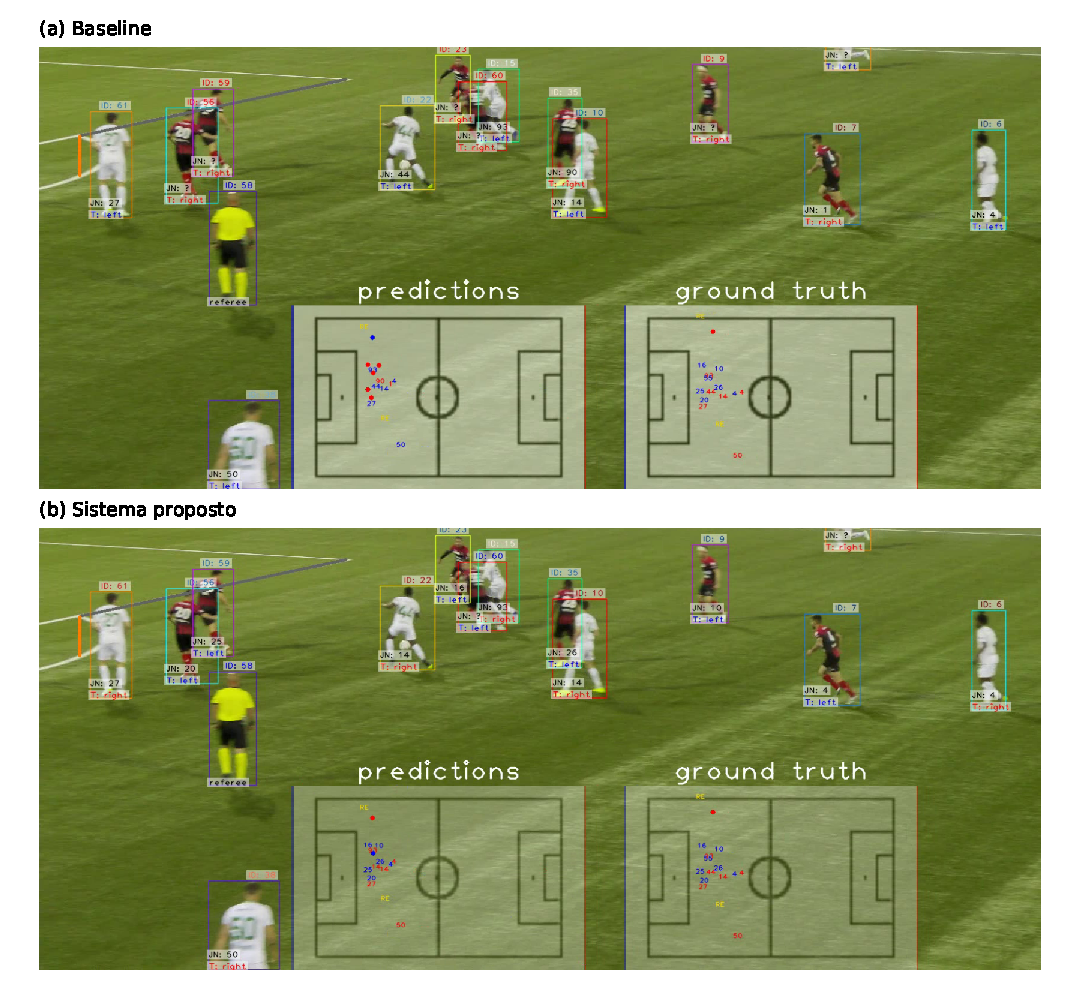
\includegraphics[width=\textwidth]{fig_frames_148.pdf}
    \caption{O mesmo \emph{frame} do SNGS-148 nos dois sistemas, tal como sai do \emph{pipeline}. Em cada mapa, as predições estão à esquerda e a anotação à direita, com \emph{left} a azul e \emph{right} a vermelho.}
    \label{fig:frames-148}
\end{figure}

\begin{figure}[H]
    \centering
    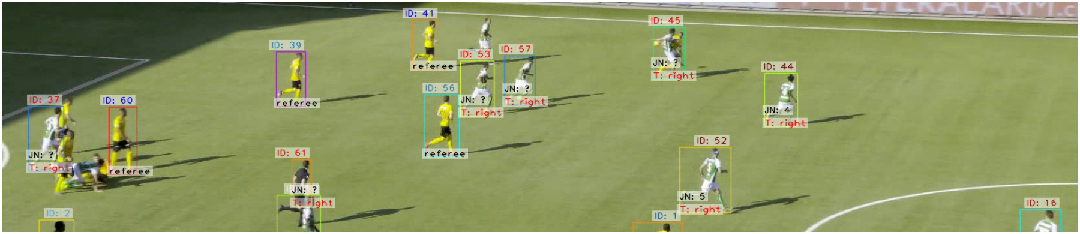
\includegraphics[width=\textwidth]{fig_arbitragem_050.pdf}
    \caption{Função atribuída no SNGS-050 pelo sistema proposto. A \emph{baseline} falha da mesma forma.}
    \label{fig:arbitragem-050}
\end{figure}

\subsection{Contributo de Cada Alteração}\label{sec:res_equipa_ablacao}\label{sec:res_equipa_degenerada}

O módulo de equipa do sistema proposto difere do da \emph{baseline} em três alterações. As duas primeiras foram medidas durante o desenvolvimento, uma de cada vez, sobre os $39$ vídeos de teste usados nessa fase (Tabela~\ref{tab:team-resultados}). A primeira junta o agrupamento pela cor, usado quando o ReID não separa as equipas, e a cascata de votação para o lado (Secções~\ref{sec:agrupamento} e~\ref{sec:mapeamento}). Sozinha, leva a exatidão de $85.4\%$ para $96.1\%$, mas estraga um vídeo, o SNGS-195, que passa de $100\%$ para $0\%$. Neste vídeo, as posições médias das duas equipas diferem apenas $0.01$ metros, e nenhum critério de posição consegue decidir. A segunda alteração, o desempate pelo guarda-redes, repara-o e leva a exatidão a $97.8\%$.

\begin{table}[H]
    \centering
    \caption{Exatidão da equipa e do lado depois de cada alteração, nos $39$ vídeos de teste usados durante o desenvolvimento.}
    \label{tab:team-resultados}
    \begin{tabular}{|l|c|c|}
        \hline
        \textbf{Estado do sistema} & \textbf{Exatidão} & \textbf{$\Delta$} \\
        \hline
        \emph{Baseline}                                   & $85.4\%$ ($1499/1755$) & --- \\
        \hline
        + agrupamento pela cor e cascata de votação       & $96.1\%$ ($1686/1755$) & $+10.7$ pp \\
        \hline
        + desempate pelo guarda-redes           & $97.8\%$ ($1717/1755$) & $+1.7$ pp \\
        \hline
    \end{tabular}
\end{table}

A terceira alteração veio depois, já com os $159$ vídeos avaliados. Nessa versão, o agrupamento tinha uma falha própria. Em onze vídeos, punha quase todos os jogadores no mesmo grupo, como se em campo houvesse uma só equipa. É o agrupamento colapsado da Tabela~\ref{tab:visual}. Nesse caso, só acertam os jogadores do lado atribuído ao grupo grande, e a exatidão fica perto de $50\%$. Em nove dos onze vídeos, ficava entre $43.6\%$ e $61.4\%$.

Esta falha deteta-se sem a anotação. Nos onze vídeos, o grupo menor tinha entre $0.1\%$ e $7.8\%$ das deteções de jogadores. Nos outros $148$, nunca tem menos de $8.7\%$, e a mediana é de $45.8\%$. Há, portanto, uma fronteira clara entre os dois casos, e o próprio módulo pode testá-la.

Posto isto, o módulo passou a verificar cada agrupamento, como descrito na Secção~\ref{sec:agrupamento}. Se o grupo menor tem menos de $8\%$ das deteções de jogadores, o agrupamento é rejeitado. Os \emph{tracklets} são então agrupados de novo pela cor da camisola, medida nas imagens. O novo agrupamento só é aceite se cumprir duas condições. A primeira é que o grupo menor tenha pelo menos $20\%$ dos \emph{tracklets} e das deteções. A segunda é que o classificador de função não classifique como árbitros mais de um quarto dos \emph{tracklets} que dá como jogadores. Se o fizer, falta uma equipa inteira ao agrupamento, e separar por cor o que resta dividiria a outra ao meio.

A Tabela~\ref{tab:regressoes} mostra os onze vídeos em que a verificação dispara. Em cada um, o agrupamento original pôs quase todos os jogadores na mesma equipa, e o grupo menor ficou com menos de $8\%$ das deteções. O SNGS-038 é o caso extremo. O grupo menor tinha só $0.1\%$ das deteções, e o novo agrupamento pela cor dividiu os \emph{tracklets} em $28$ e $16$. A exatidão da equipa passou de $55.2\%$ para $100\%$.

\begin{table}[H]
    \centering
    \caption{Vídeos em que a verificação do agrupamento colapsado dispara.}
    \label{tab:regressoes}
    \begin{tabular}{|l|c|c|c|c|c|}
        \hline
         & \textbf{Agrupamento rejeitado} & \textbf{Novo agrupamento} & \multicolumn{3}{c|}{\textbf{Exatidão da equipa}} \\
        \cline{2-6}
        \textbf{Vídeo} & \textbf{\begin{tabular}[c]{@{}c@{}}Deteções no\\ grupo menor\end{tabular}} & \textbf{\begin{tabular}[c]{@{}c@{}}\emph{Tracklets}\\ por grupo\end{tabular}} & \textbf{\emph{Baseline}} & \textbf{Antes} & \textbf{Depois} \\
        \hline
        SNGS-025 & $3.9\%$ & $33/46$ & $100.0\%$ & $61.4\%$ & $100.0\%$ \\
        \hline
        SNGS-027 & $2.8\%$ & $37/40$ & $52.2\%$ & $47.8\%$ & $100.0\%$ \\
        \hline
        SNGS-028 & $5.9\%$ & $26/27$ & $54.5\%$ & $54.5\%$ & $100.0\%$ \\
        \hline
        SNGS-030 & $0.5\%$ & $31/14$ & $40.0\%$ & $60.0\%$ & $100.0\%$ \\
        \hline
        SNGS-036 & $3.3\%$ & $19/24$ & $96.8\%$ & $51.6\%$ & $100.0\%$ \\
        \hline
        SNGS-038 & $0.1\%$ & $28/16$ & $100.0\%$ & $55.2\%$ & $100.0\%$ \\
        \hline
        SNGS-091 & $7.8\%$ & $33/37$ & $86.7\%$ & $57.8\%$ & $97.8\%$ \\
        \hline
        SNGS-131 & $7.1\%$ & $29/40$ & $0.0\%$ & $43.6\%$ & $0.0\%$ \\
        \hline
        \multicolumn{6}{|l|}{\emph{Novo agrupamento recusado}} \\
        \hline
        SNGS-039 & $5.8\%$ & --- & $21.9\%$ & $0.0\%$ & $0.0\%$ \\
        \hline
        SNGS-050 & $0.8\%$ & --- & $60.9\%$ & $100.0\%$ & $100.0\%$ \\
        \hline
        SNGS-069 & $2.7\%$ & --- & $100.0\%$ & $53.3\%$ & $53.3\%$ \\
        \hline
    \end{tabular}
\end{table}

Em oito vídeos o novo agrupamento é aceite, e a inspeção visual confirma que as duas equipas ficam bem separadas. Seis chegam a $100\%$ e o SNGS-091 a $97.8\%$. O SNGS-131 desce para $0\%$, mas só porque a anotação deste vídeo tem os lados trocados (Secção~\ref{sec:res_equipa_resultados}). Nos outros três, o novo agrupamento é recusado e nada muda. Nos restantes $148$ vídeos, a verificação não dispara.

Os três recusados têm causas diferentes. No SNGS-039 e no SNGS-050, os jogadores de amarelo estão classificados como árbitros. Falta uma equipa ao agrupamento, e a segunda condição impede que a cor divida a outra ao meio. Os $100\%$ do SNGS-050 são enganadores, porque a métrica só avalia a equipa que sobra. No SNGS-069, as equipas jogam de verde e de branco. Ao excluir os píxeis de relva, o descritor de cor apaga também parte das camisolas verdes, e o novo agrupamento volta a ficar desequilibrado. Num ensaio à parte, uma máscara do fundo estimada em cada recorte separou bem as duas equipas, e fica como trabalho futuro.

\subsection{Onde o Sistema Proposto Ainda piora}\label{sec:res_equipa_regressoes}\label{sec:res_equipa_metrica}

Mesmo com as três alterações, o sistema proposto fica abaixo da \emph{baseline} em $11$ vídeos. Cinco são do bloco da equipa de amarelo (SNGS-039, 042, 052, 055 e 057). Aí, os dois sistemas classificam os jogadores de amarelo como árbitros, e o resultado depende de como cada um divide a equipa que fica. Outro é o SNGS-069, o vídeo de verde e branco descrito acima, que continua com o agrupamento colapsado. Há ainda o SNGS-113, com as equipas bem separadas mas o lado trocado. Nos quatro restantes, a diferença é de um a três \emph{tracklets} na equipa errada. Apesar destas descidas, o GS-HOTA sobe em sete dos onze vídeos, e em todos eles o número também melhora.

O SNGS-113 foi analisado na Secção~\ref{sec:mapeamento}. As duas equipas jogam na mesma metade do campo, e o lado é decidido pela votação relativa, o segundo critério da cascata, com uma diferença de $15$ pontos. A média das posições, que a \emph{baseline} usa, acertaria. Mas a cascata só a consulta no terceiro critério, e este vídeo não chega lá.

Por fim, há três vídeos que pioram sem que a métrica o mostre. No SNGS-023 e no SNGS-187, um \emph{tracklet} segue dois jogadores de equipas opostas, quase metade do tempo cada um, e por isso mostra a equipa errada durante parte do vídeo. A exatidão por \emph{tracklet} exclui os \emph{tracklets} que trocam de jogador, e por isso dá $100\%$ aos dois sistemas. No SNGS-197, o sistema proposto troca o lado, e a anotação invertida dá-lhe $100\%$.

\subsection{Robustez do Critério de Atribuição do Lado}\label{sec:res_lado_quantificacao}

Como se viu na Secção~\ref{sec:equipa-desafio}, a maioria das soluções apresentadas ao desafio decide o lado do campo pela posição horizontal média dos jogadores de cada equipa. Nenhuma mede com que frequência esta regra falha. Essa medição foi feita aqui diretamente sobre a anotação, para separar o comportamento da regra dos erros dos outros módulos. Como não depende do sistema, abrange os $160$ vídeos, incluindo o SNGS-096, que fica fora das restantes comparações porque a calibração falha nele.


Compararam-se dois critérios com o lado anotado (Tabela~\ref{tab:lado-inversoes}). O primeiro é a posição do guarda-redes, que não acompanha as fases de ataque e fica junto da sua baliza. Nos $156$ vídeos em que aparece, a sua posição nunca contradiz o lado que lhe foi anotado. O segundo é a posição média dos jogadores de campo de cada equipa. Esta regra discorda da anotação em $7$ dos $160$ vídeos, mas só em dois erra de facto. No SNGS-038 e no SNGS-195, as duas equipas ocupam quase a mesma zona do campo, e as suas posições médias diferem menos de um metro. Os outros cinco são os vídeos com a anotação invertida descritos na Secção~\ref{sec:res_equipa_resultados}. Neles, a regra indica o lado verdadeiro, e é a anotação que está errada. Com a mediana em vez da média, a regra discorda em nove vídeos, porque junta aos sete anteriores o SNGS-056 e o SNGS-130. Usa-se, por isso, a média, que é também a formulação habitual na literatura.

\begin{table}[H]
    \centering
    \caption{Concordância de dois critérios com o lado anotado, nos $160$ vídeos dos três subconjuntos.}
    \label{tab:lado-inversoes}
    \begin{tabular}{|l|c|c|c|}
        \hline
        \textbf{Critério} & \textbf{Vídeos avaliáveis} & \textbf{Discorda da anotação} & \textbf{Dos quais, anotação invertida} \\
        \hline
        Posição do guarda-redes  & $156$ & $0$ & $0$ \\
        \hline
        Posição média da equipa  & $160$ & $7$ ($4.4\%$) & $5$ \\
        \hline
    \end{tabular}
\end{table}

Os dois casos reais mostram o ponto fraco da regra. Quando as duas equipas estão na mesma zona do campo, as médias quase coincidem e a sua ordem deixa de indicar o lado. É este cenário que a cascata da Secção~\ref{sec:mapeamento} trata à parte, primeiro com as votações e, no fim, com o guarda-redes. Ensaiou-se ainda substituir a posição média pelo jogador de campo mais recuado de cada equipa. A ideia é que a última linha defensiva fica entre os atacantes e a sua baliza. Sobre a anotação, este critério só concorda com o lado anotado em $68.6\%$ dos vídeos, contra $95.6\%$ da posição média. A câmara mostra apenas parte do campo, e o jogador mais recuado que se vê nem sempre é o último defesa. A alternativa foi, por isso, posta de parte.

\section{Desempenho Global}\label{sec:desempenho_global}\label{sec:desempenho-global}

O sistema completo é avaliado com o GS-HOTA, a métrica oficial do desafio (Secção~\ref{sec:protocolo}). As secções anteriores mediram cada módulo isoladamente. O GS-HOTA depende também da posição de cada jogador no campo, que vem da calibração da câmara e não faz parte das alterações deste trabalho. Ao calcular o GS-HOTA, encontrou-se na \emph{baseline} um defeito de calibração que piorava as suas posições. Sem o corrigir, parte da diferença entre os dois sistemas seria atribuída ao sistema proposto sem lhe pertencer. A Secção~\ref{sec:res_calib_defeito} descreve o defeito e a sua correção, e as seguintes apresentam os resultados.

\subsection{Correção da Calibração da \emph{Baseline}}\label{sec:res_calib_defeito}

Os dois sistemas usam as mesmas deteções, o mesmo \emph{tracking} e o mesmo código de calibração. Por isso, o GS-HOTA calculado só com a posição, sem os atributos, devia ser igual nos dois. Na primeira avaliação não era. No conjunto de teste, deu $56.7\%$ na \emph{baseline} e $61.8\%$ no sistema proposto. Ao comparar a posição no campo de cada deteção, viu-se que os dois sistemas só coincidiam no primeiro \emph{frame} de cada lote de oito. A causa está na configuração por omissão da \emph{baseline}, que calibra a câmara em lotes de oito \emph{frames}. O módulo de calibração lê os pontos do campo apenas do primeiro \emph{frame} de cada lote e aplica a mesma homografia aos outros sete. Quando a câmara se move dentro do lote, as posições desses sete \emph{frames} ficam erradas. O sistema proposto processa a calibração com lotes de um só \emph{frame}, para caber na memória da placa gráfica junto com o Qwen. Calcula assim uma homografia para cada \emph{frame}, e por isso não tem este defeito.

Para comparar os dois sistemas nas mesmas condições, a calibração da \emph{baseline} foi corrigida da mesma forma, com uma homografia própria para cada \emph{frame} em vez de uma por lote. Os pontos do campo já detetados foram reaproveitados, e só a homografia foi calculada de novo. Com as novas posições, o lado de cada equipa foi depois recalculado com o módulo original da \emph{baseline}. Esta correção não faz parte do sistema proposto nem é um contributo deste trabalho. Serve apenas para que a diferença entre os dois sistemas meça as alterações feitas, e não um defeito de configuração. Todos os valores da \emph{baseline} neste capítulo, incluindo os das Secções~\ref{sec:res_jnr} e~\ref{sec:res_equipa}, são os da versão corrigida. No conjunto de teste, o defeito custava à \emph{baseline} cerca de $5$ pontos no GS-HOTA só com a posição, e $2.4$ na métrica completa. A correção pode, por isso, ser útil a quem use a \emph{baseline} na configuração por omissão, mas esse não foi o seu objetivo.

\subsection{GS-HOTA por Subconjunto}\label{sec:res_gshota}

A Tabela~\ref{tab:gshota} mostra o GS-HOTA dos dois sistemas nos três subconjuntos, com as suas três componentes. A DetA mede a deteção, a AssA a associação ao longo do tempo e a LocA a exatidão da posição. O sistema proposto obtém $47.87\%$ no teste, $36.79\%$ na validação e $45.37\%$ no treino. A \emph{baseline} obtém $31.30\%$, $23.68\%$ e $31.52\%$. Os ganhos são de $16.57$, $13.11$ e $13.85$ pontos.

\begin{table}[H]
    \centering
    \caption{GS-HOTA e componentes nos três subconjuntos. A \emph{baseline} é a versão com a calibração corrigida (Secção~\ref{sec:res_calib_defeito}).}
    \label{tab:gshota}
    \begin{tabular}{|l|l|c|c|c|c|}
        \hline
        \textbf{Conjunto} & \textbf{Sistema} & \textbf{GS-HOTA} & \textbf{DetA} & \textbf{AssA} & \textbf{LocA} \\
        \hline
        \multirow{2}{*}{Teste}     & \emph{Baseline}  & $31.30\%$ & $17.5$ & $56.1$ & $92.8$ \\
        \cline{2-6}
                                   & Sistema proposto & $47.87\%$ & $39.0$ & $58.7$ & $93.3$ \\
        \hline
        \multirow{2}{*}{Validação} & \emph{Baseline}  & $23.68\%$ & $10.3$ & $54.4$ & $91.5$ \\
        \cline{2-6}
                                   & Sistema proposto & $36.79\%$ & $24.5$ & $55.3$ & $92.3$ \\
        \hline
        \multirow{2}{*}{Treino}    & \emph{Baseline}  & $31.52\%$ & $17.9$ & $55.6$ & $92.0$ \\
        \cline{2-6}
                                   & Sistema proposto & $45.37\%$ & $36.3$ & $56.7$ & $92.2$ \\
        \hline
    \end{tabular}
\end{table}

Quase todo o ganho está na DetA, que sobe entre $14.2$ e $21.5$ pontos. A AssA e a LocA mudam menos de $3$ pontos. É o que se espera, porque o GS-HOTA só conta uma deteção como certa se a função, a equipa e o número também estiverem certos. São estes atributos que o sistema proposto melhora, e não a deteção nem a posição, que são iguais nos dois sistemas. O ganho tem a mesma ordem de grandeza nos três subconjuntos, por isso não depende de um subconjunto em particular.

Por vídeo, o ganho mediano é de $15.0$ pontos no teste, $15.5$ na validação e $14.0$ no treino. Só seis vídeos ficam mais de um ponto abaixo da \emph{baseline}. Quatro são regressões da equipa, já descritas na Secção~\ref{sec:res_equipa_regressoes} (SNGS-039, 042, 069 e 113). Os outros dois, o SNGS-043 e o SNGS-049, são do bloco da equipa de amarelo, em que a falha da função domina o resultado dos dois sistemas.

\subsection{Decomposição por Atributo}\label{sec:res_decomposicao}

O GS-HOTA junta todos os módulos num só valor, porque uma deteção só conta se a função, a equipa e o número também estiverem certos. Para separar o efeito de cada atributo, a métrica foi recalculada com os atributos acrescentados um a um. Primeiro conta só a posição no campo, depois junta-se a função, a equipa e, por fim, o número. A última coluna da Tabela~\ref{tab:decomposicao} é, assim, a métrica oficial. A solução vencedora de 2025 fez uma análise parecida (Secção~\ref{sec:jnr-desafio}), mas com cada atributo isolado e só para o seu próprio sistema.

\begin{table}[htbp]
    \centering
    \caption{GS-HOTA com os atributos acrescentados um a um. A última coluna é a métrica oficial.}
    \label{tab:decomposicao}
    \begin{tabular}{|l|l|c|c|c|c|}
        \hline
        \textbf{Conjunto} & \textbf{Sistema} & \textbf{Posição} & \textbf{+ função} & \textbf{+ equipa} & \textbf{+ número} \\
        \hline
        \multirow{2}{*}{Teste}     & \emph{Baseline}  & $61.8$ & $59.4$ & $53.8$ & $31.3$ \\
        \cline{2-6}
                                   & Sistema proposto & $61.8$ & $59.4$ & $57.4$ & $47.9$ \\
        \hline
        \multirow{2}{*}{Validação} & \emph{Baseline}  & $57.7$ & $47.4$ & $38.5$ & $23.7$ \\
        \cline{2-6}
                                   & Sistema proposto & $57.7$ & $47.4$ & $43.0$ & $36.8$ \\
        \hline
        \multirow{2}{*}{Treino}    & \emph{Baseline}  & $58.3$ & $58.2$ & $56.1$ & $31.5$ \\
        \cline{2-6}
                                   & Sistema proposto & $58.3$ & $58.2$ & $55.8$ & $45.4$ \\
        \hline
    \end{tabular}
\end{table}

Só com a posição, os dois sistemas dão o mesmo valor, como têm de dar. Esse valor, entre $57.7\%$ e $61.8\%$, é o máximo que o GS-HOTA pode atingir com a deteção, o \emph{tracking} e a calibração atuais. A função também não foi alterada e custa o mesmo aos dois sistemas. Na validação custa $10.3$ pontos, contra $2.4$ no teste e $0.1$ no treino, por causa dos $20$ vídeos da equipa de amarelo.

A equipa e o número, os dois atributos alterados, são os que afastam os dois sistemas. No teste, a equipa custa $5.6$ pontos à \emph{baseline} e $2.0$ ao sistema proposto. O número tira-lhes $22.5$ e $9.5$. Dos $16.6$ pontos de ganho no teste, $3.6$ vêm da equipa e $13.0$ do número. Na validação, dos $13.1$ pontos, $4.5$ vêm da equipa e $8.6$ do número. No treino, dos $13.9$ pontos, o número dá $14.2$ e a equipa tira $0.3$.

O número é o atributo que mais custa, nos dois sistemas e nos três conjuntos. A única exceção é a validação do sistema proposto, onde a função custa mais do que o número ($10.3$ contra $6.2$ pontos), por causa da equipa com equipamento amarelo. Isto confirma com a métrica oficial o que a solução vencedora de 2025 concluiu sobre o seu sistema, em que o número é também o principal ponto fraco.

\subsection{Enquadramento Competitivo}\label{sec:res_leaderboard}

Os valores deste trabalho não são diretamente comparáveis com a classificação oficial do desafio. Essa classificação é feita no conjunto \emph{challenge}, cuja anotação não é pública, e não nos conjuntos usados aqui. Ainda assim, a Tabela~\ref{tab:leaderboard} dá uma ordem de grandeza, com os três melhores sistemas e a \emph{baseline} oficial de cada edição. A \emph{baseline} oficial de 2025 obtém $29.01\%$ no \emph{challenge}. A mesma \emph{baseline}, corrida neste trabalho na configuração por omissão, obtém $28.95\%$ no teste. Os dois valores são próximos, o que dá alguma confiança na reprodução.

\begin{table}[H]
    \centering
    \caption{Três melhores sistemas e \emph{baseline} oficial das edições de 2024 e 2025, no conjunto \emph{challenge} \citep{cioppa2024soccernet, giancola2025soccernet}.}
    \label{tab:leaderboard}
    \begin{tabular}{|l|c|}
        \hline
        \textbf{Sistema} & \textbf{GS-HOTA} \\
        \hline
        \multicolumn{2}{|l|}{\textit{Edição de 2024}} \\
        \hline
        Constructor Tech  & $63.81\%$ \\
        \hline
        UPCxMobius        & $43.15\%$ \\
        \hline
        JAM               & $34.40\%$ \\
        \hline
        \emph{Baseline} oficial & $23.36\%$ \\
        \hline
        \multicolumn{2}{|l|}{\textit{Edição de 2025}} \\
        \hline
        KIST-GSR          & $63.90\%$ \\
        \hline
        Constructor Tech  & $63.81\%$ \\
        \hline
        lianyou           & $62.76\%$ \\
        \hline
        \emph{Baseline} oficial & $29.01\%$ \\
        \hline
    \end{tabular}
\end{table}

Os sistemas do topo passam os $60\%$ com melhorias em todo o \emph{pipeline}, incluindo a deteção e a calibração. Este trabalho não alterou nenhuma destas duas partes. Só com a posição, antes de contar qualquer atributo, o sistema proposto fica em $61.8\%$ no teste (Tabela~\ref{tab:decomposicao}). Esse é o máximo que pode atingir enquanto a deteção e a calibração forem as da \emph{baseline}.

O sistema proposto tem três pontos em comum com estas soluções. A vencedora de 2025 \citep{oo2026broadcast2pitch} usa um modelo de visão e linguagem, o LLaMA-3.2-Vision, para ler a função, o número e a cor de cada jogador. O sistema proposto faz o mesmo com o Qwen, mas só para o número. O relatório dessa edição \citep{giancola2025soccernet} refere também o Qwen2-VL entre os modelos usados com sucesso para esta leitura. A mesma solução agrupa os jogadores pela cor da camisola, como o sistema proposto. Mas decide o lado pela média das posições, que é a regra da \emph{baseline} que a cascata deste trabalho substitui. Por fim, o recorte do tronco guiado pela pose, que antecede a leitura do número, também aparece noutra solução da edição de 2025.


\section{Custo Computacional}\label{sec:res_tempos}

A Tabela~\ref{tab:tempos} mostra o tempo de cada módulo por vídeo de $30$ segundos ($750$ \emph{frames}), na GPU portátil descrita na Secção~\ref{sec:ambiente}. Os valores são medianas sobre os vídeos processados, medidas pelo cronómetro do próprio motor de execução. O total é de $21.3$ minutos na \emph{baseline} e $22.0$ no sistema proposto, muito longe do tempo real. Nos dois sistemas, a maior parte do tempo vai para a reidentificação, a leitura do número e a deteção dos pontos do campo. A redução deste custo é discutida no Capítulo~\ref{cap:conclusao}.

\begin{table}[htbp]
    \centering
    \caption{Tempo de execução de cada módulo num vídeo de $750$ \emph{frames}, em segundos. Mediana sobre os vídeos processados.}
    \label{tab:tempos}
    \begin{tabular}{|l|c|c|}
        \hline
        \textbf{Módulo} & \textbf{\emph{Baseline}} & \textbf{Sistema proposto} \\
        \hline
        Deteção (YOLOv8)                          & $97.3$  & $96.4$ \\
        \hline
        Reidentificação (PRTreID)                 & $448.7$ & $484.4$ \\
        \hline
        \emph{Tracking} (StrongSORT)              & $31.8$  & $30.9$ \\
        \hline
        Pontos do campo (NBJW)                    & $211.9$ & $210.3$ \\
        \hline
        Calibração (homografia)                   & $5.7$   & $21.5$ \\
        \hline
        Número da camisola (MMOCR / proposto)     & $486.7$ & $477.7$ \\
        \hline
        Voto por \emph{tracklet}                  & $0.1$   & $0.1$ \\
        \hline
        Equipa (agrupamento)                      & $0.7$   & $1.3$ \\
        \hline
        Lado do campo                             & $0.0$   & $0.1$ \\
        \hline
        Total dos módulos                         & $21.3$ min & $22.0$ min \\
        \hline
    \end{tabular}
\end{table}

As alterações deste trabalho acrescentam pouco tempo. No sistema proposto, o reconhecimento do número da camisola demora o mesmo que com o MMOCR, $478$ contra $487$ segundos, apesar de usar um modelo de visão e linguagem. Isto acontece porque só lê os recortes que passam o filtro de qualidade. O agrupamento e o lado do campo somam menos de dois segundos por vídeo. A maior diferença está na reidentificação, que demora mais $36$ segundos porque, no sistema proposto, calcula também o descritor de cor da camisola usado no agrupamento. A calibração passa de $5.7$ para $21.5$ segundos, porque o sistema proposto calcula uma homografia por \emph{frame} e a \emph{baseline} uma por lote de oito (Secção~\ref{sec:res_calib_defeito}).

A decisão pela confiança obrigou ainda a ler cada janela uma segunda vez, para registar as probabilidades dos \emph{tokens}. Esta segunda leitura correu à parte do \emph{pipeline}, não foi cronometrada e não está incluída na tabela. As probabilidades saem da mesma chamada ao modelo que gera a resposta, e por isso podem ser registadas logo na primeira leitura. Numa implementação integrada, este custo desaparece.

\section{Síntese}\label{sec:res_sintese}

Este trabalho alterou quatro dos nove módulos da \emph{baseline}. Substituiu ou reescreveu três, o reconhecimento do número da camisola, a equipa e o lado do campo, e estendeu um, a reidentificação. O ganho é claro e repete-se nos três subconjuntos.

O reconhecimento do número da camisola passa de $15.3\%$ para $42.6\%$ dos \emph{tracklets} nos $159$ vídeos. Melhora em $156$ vídeos e não piora em nenhum. A decisão pela confiança da leitura reduz os números errados a cerca de um terço, de $12.3\%$ para $4.4\%$. A atribuição da equipa e do lado passa de $83.5\%$ para $92.8\%$. Na inspeção visual, os vídeos com falhas deste módulo descem de $28$ para $7$. No GS-HOTA, o ganho é de $16.57$ pontos no teste, $13.11$ na validação e $13.85$ no treino. A decomposição por atributo mostra que todo este ganho vem da equipa e do número, os dois atributos alterados.

A comparação foi feita contra a \emph{baseline} com a calibração corrigida. Sem essa correção, o defeito de calibração custava-lhe cerca de $5$ pontos de GS-HOTA na posição e $2.4$ na métrica completa, que passariam por ganho do sistema proposto.

Os limites também ficaram claros. Nos casos mais difíceis, o número não está visível na imagem devido à distância da câmara ou à orientação do jogador, e nenhuma transformação do recorte o recupera (Secção~\ref{sec:res_jnr_teto}). Na atribuição da equipa, ficam $20$ vídeos em que o classificador de função, que não foi alterado, dá todos os jogadores de amarelo como árbitros. Ficam também três vídeos com o lado trocado, um deles comum aos dois sistemas. Numa versão anterior, o sistema proposto juntava por vezes quase todos os jogadores num só grupo. A verificação da Secção~\ref{sec:res_equipa_degenerada} corrige oito dos onze vídeos em que isso acontecia e não muda nenhum dos outros $148$.